\chapter{The smoothness assumption in the global algorithm}
The last part of our work focuses on the addition of the smoothness constraint to the overall algorithm described in chapter \ref{sec:GD}.
\section{Results}
Again, the starting conditions for the experiments are analogues to the ones supposed in chapters \ref{sec:GD} and \ref{sec:DL}, the number of iterations is, again, $250$ and there is still a rate $5:1$ for the number of iterations dedicated to the graph learning part, per each iteration dedicated to the dictionary learning one.
\\

The figures \ref{fig:alphaHeatGD_smth} and \ref{fig:alphaDorinaGD_smth} show the comparison between the kernels learned without and with the smoothness assumption. In both the figures we see how the smoothness assumption still improves the kernel learning process, at the same time respecting the overall spectral composition of the signal.

\begin{figure}
  \centering
  \begin{minipage}[c]{.8\textwidth}
    \centering
    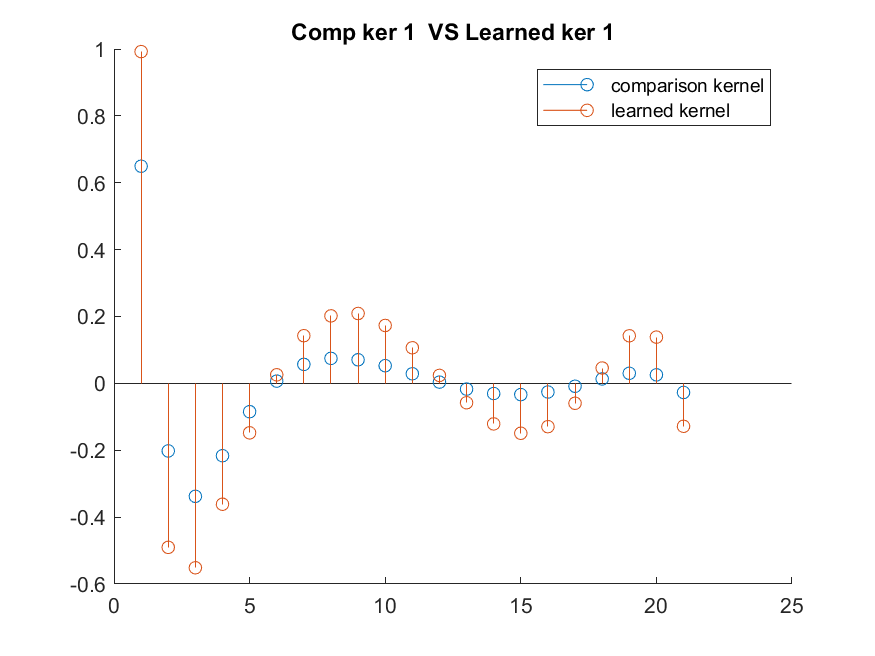
\includegraphics[width = \textwidth]{alphaDorina_noSmoothness_dictionary.png}
  \end{minipage}
  \begin{minipage}[c]{.8\textwidth}
    \centering
    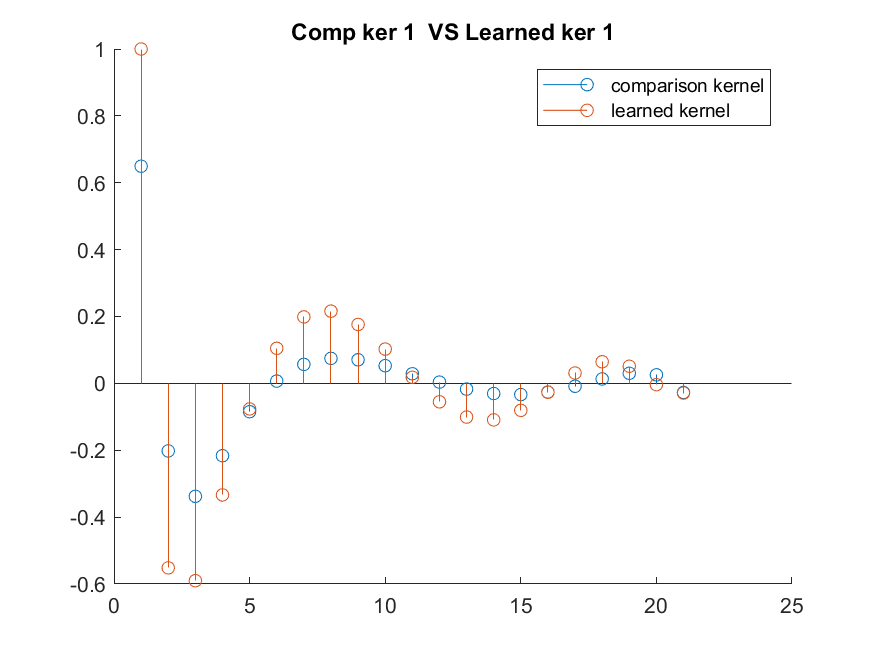
\includegraphics[width = \textwidth]{alphaDorina_Smoothness_dictionary.png}
  \end{minipage}
  \caption{Comparison between kernels coefficients without and with smoothness prior. Thanou et al.   dataset}
  \label{fig:alphaHeatGD_smth}
\end{figure}

\begin{figure}
  \centering
  \begin{minipage}[c]{.8\textwidth}
    \centering
    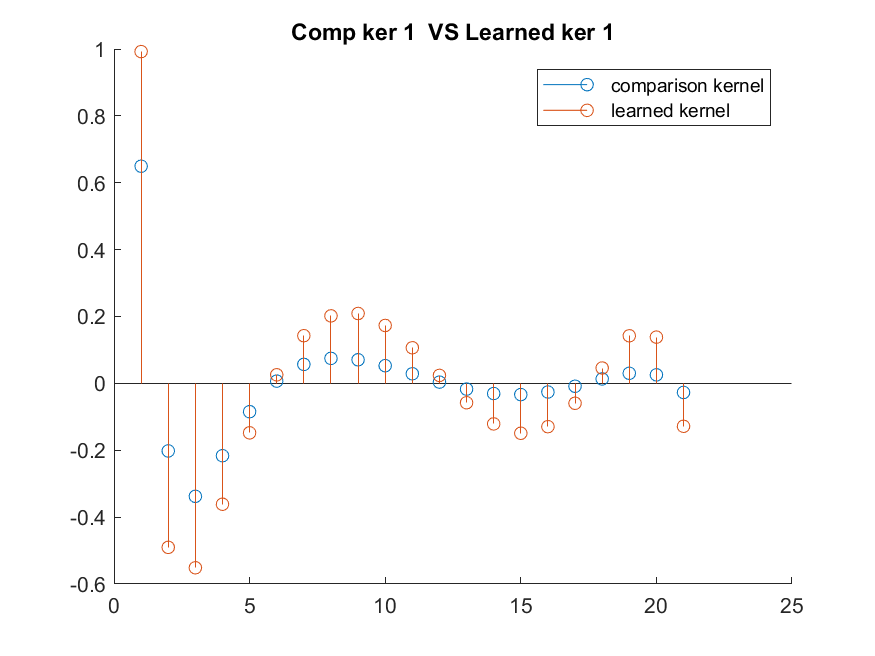
\includegraphics[width = \textwidth]{alphaDorina_noSmoothness_dictionary.png}
  \end{minipage}
  \begin{minipage}[c]{.8\textwidth}
    \centering
    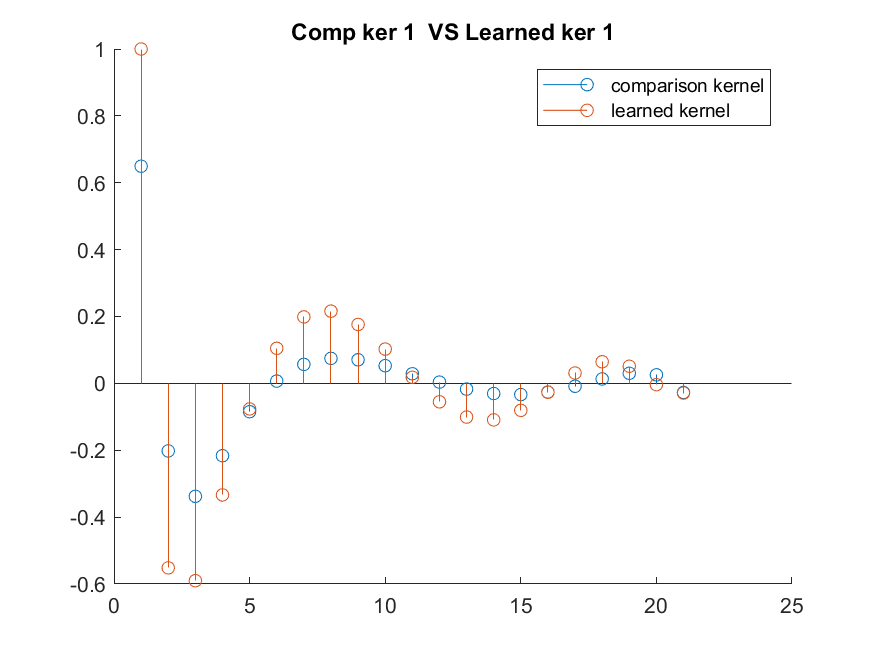
\includegraphics[width = \textwidth]{alphaDorina_Smoothness_dictionary.png}
  \end{minipage}
  \caption{Comparison between kernels coefficients without and with smoothness prior. Thanou et al.   dataset}
  \label{fig:alphaDorinaGD_smth}
\end{figure}

Table \ref{tab:PrecRec_compSmth} again shows the comparison between the Precision and Recall values obtained from the approach without the smoothness prior and the approach accounting for it. The values listed clearly show how the algorithm benefits from the prior, having both the values increased. We emphasize that the value listed in the table is an average of repeated trials, but if we have a look into the general behavior of the algorithm through several attempts, it stands out how the behavior of the algorithm appears to be stable, as shown in \autoref{tab:PrecRec_repetitions}.

\begin{table}[htbp]
  \centering
  \begin{tabular}{lcccc}
  &\multicolumn{2}{c}{\textbf{Heat kernel}}&\multicolumn{2}{c}{\textbf{Thanou et al. kernel}}\\
  \toprule
  &Graph L. & Graph and D. L. & Graph L. & Graph and D. L.\\ %\cline{2-5}
    \midrule
    \textbf{Precision rate} & 0 & 0 & 0 & 0\\
    \textbf{Recall Rate} & 0 & 0 & 0 & 0\\
    \bottomrule
  \end{tabular}
  \caption{Reproduction error comparison for the low frequency kernel from Thanou et al. dataset}
  \label{tab:PrecRec_compSmth}
\end{table}

\begin{table}[htbp]
  \centering
  \begin{tabular}{ccc}
  \textbf{Trial \#} & \textbf{Heat kernel} & \textbf{Thanou et al. kernel}\\
  \midrule
    0 & 0\\
    0 & 0\\
    \bottomrule
  \end{tabular}
  \caption{Reproduction error comparison for the low frequency kernel from Thanou et al. dataset}
  \label{tab:PrecRec_repetitions}
\end{table}

Finally, for what concerns the kernels coefficients, figures \ref{fig:alphaGDHeat} and \ref{fig:alphaGDDorina} highlight one time more how the smoothness prior has a good repercussion over them, allowing to get more faithful behaviors.

\begin{figure}
  \centering
  \begin{minipage}[c]{.8\textwidth}
    \centering
    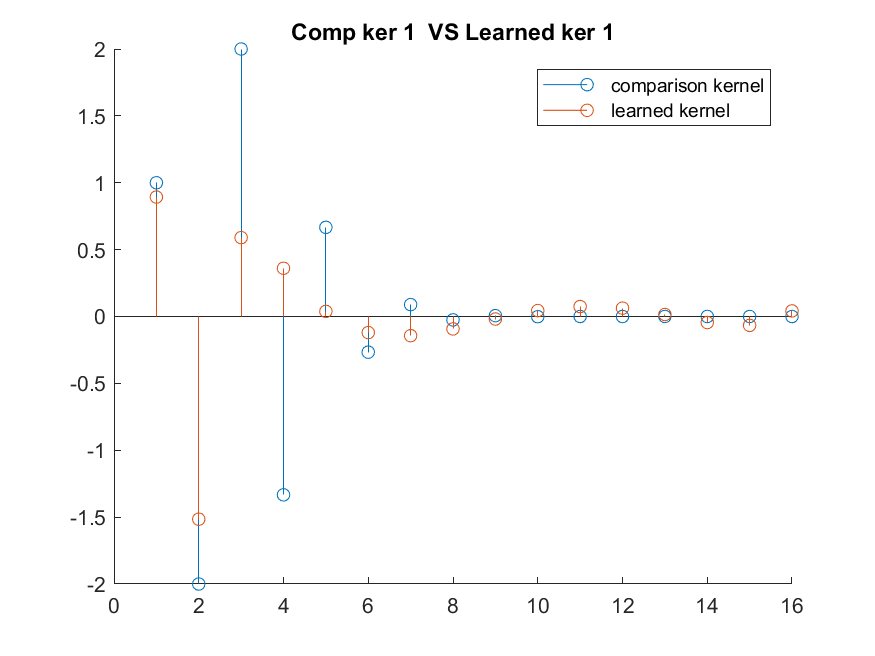
\includegraphics[width = \textwidth]{alphaHeat_noSmoothness_dictionary.png}
  \end{minipage}
  \begin{minipage}[c]{.8\textwidth}
    \centering
    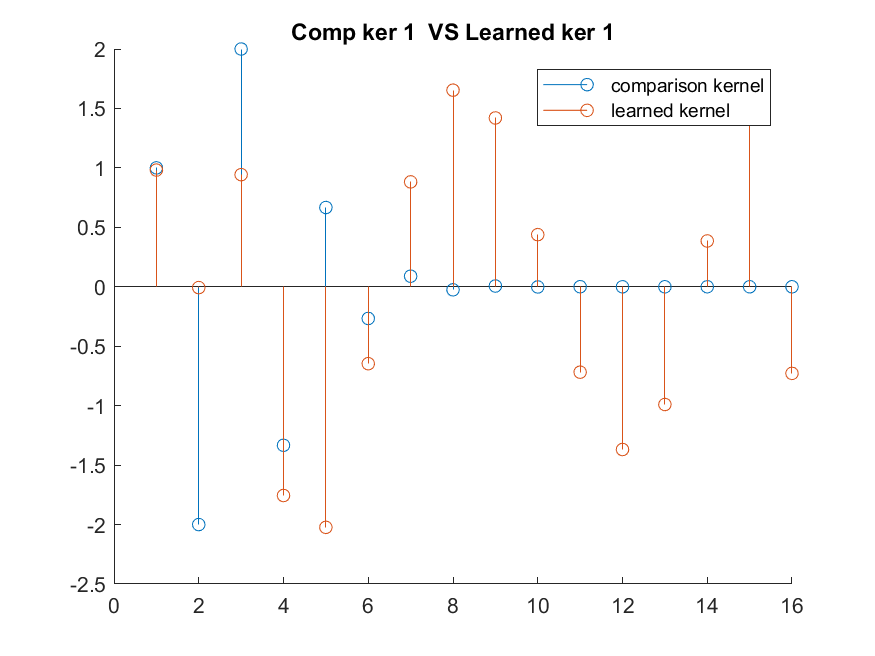
\includegraphics[width = \textwidth]{alphaHeat_Smoothness_dictionary.png}
  \end{minipage}
  \caption{Comparison between kernels coefficients without and with smoothness prior. Heat kernel   dataset}
  \label{fig:alphaGDHeat}
\end{figure}

\begin{figure}
  \centering
  \begin{minipage}[c]{.8\textwidth}
    \centering
    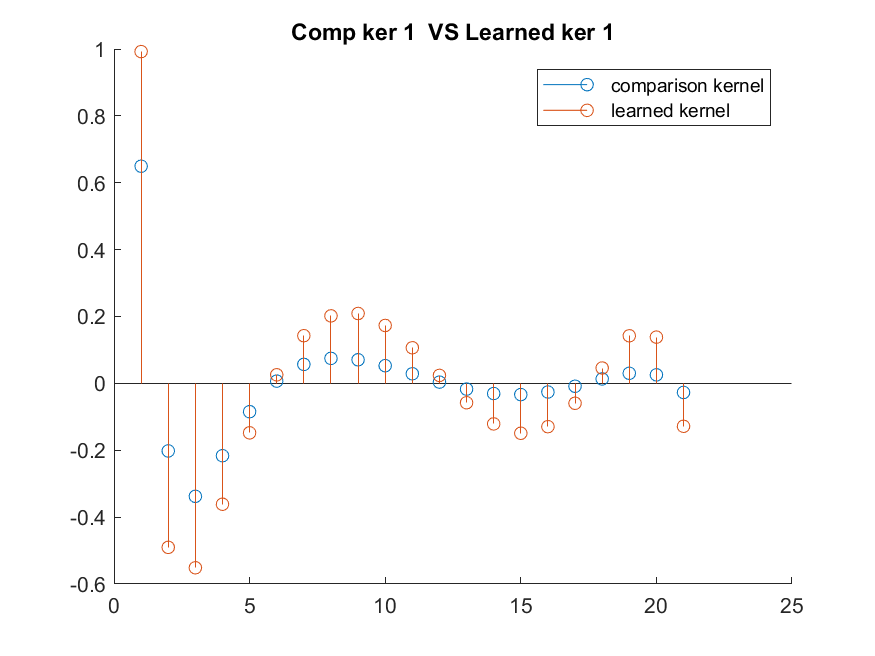
\includegraphics[width = \textwidth]{alphaDorina_noSmoothness_dictionary.png}
  \end{minipage}
  \begin{minipage}[c]{.8\textwidth}
    \centering
    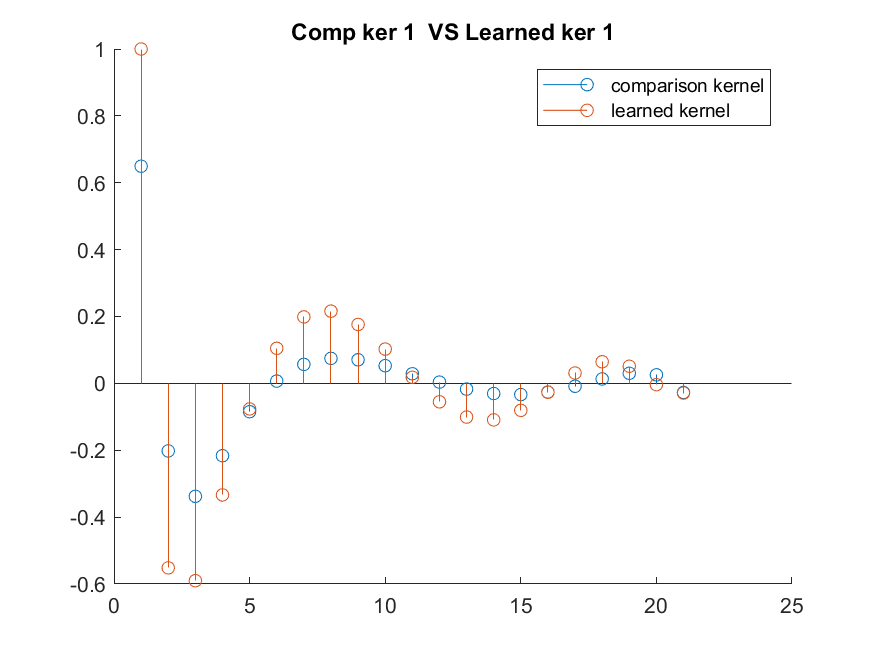
\includegraphics[width = \textwidth]{alphaDorina_Smoothness_dictionary.png}
  \end{minipage}
  \caption{Comparison between kernels coefficients without and with smoothness prior. Thanou et al.   dataset}
  \label{fig:alphaGDDorina}
\end{figure}
